\documentclass[11pt]{article}

\usepackage[margin=1.15in]{geometry}
\usepackage{amsmath,amssymb,amsthm}
\usepackage{graphicx}
\usepackage{booktabs}
\usepackage[T1]{fontenc}
\usepackage{lmodern}
\usepackage{microtype}
\usepackage[hidelinks]{hyperref}
\usepackage{caption}

\newcommand{\rt}{\widetilde{r}}
\newcommand{\gapdist}{1-\langle\rt\rangle}
\newcommand{\kstar}{k^{*}}
\newcommand{\seff}{\sigma_{\mathrm{eff}}}
\newcommand{\ssys}{\sigma_{\mathrm{sys}}}
\newcommand{\smean}{\sigma_{\mathrm{mean}}}
\newcommand{\verdict}[1]{\textsc{#1}}

\title{Local crystallization beneath a frozen global measure:\\
sealed measurements of spacing statistics\\ under repeated differentiation}
\author{}
\date{}

\emergencystretch=2.5em

\begin{document}
\maketitle

\begin{abstract}
Let $p$ be a real-rooted polynomial of degree $n$ with roots drawn from a seed ensemble, and
let $p^{(k)}$ denote its $k$-th derivative. Recent theorems prove that the \emph{global}
empirical root measure of $p^{(k)}$ is asymptotically frozen at the seed measure through every
$k=o(n)$ for real roots (Angst--Nguyen--Poly, extending Kabluchko, Byun--Lee--Reddy, and
Michelen--Vu).\footnote{Corrected 2026-08-17 on A.\ Campbell's correction: $o(n/\log n)$ is the
best known for \emph{complex} roots; for real roots the seed measure remains the limit to
$o(n)$. The earlier text quoted the complex-root bound for our real-rooted seeds, understating
the window over which the global measure is frozen --- i.e.\ understating the two-scale
contrast.} We measure what happens beneath that frozen profile: the \emph{local spacing
statistics}, for which, to our knowledge, no theorem and no prior measurement exists in any
regime $1\ll k\le sn$, $s<1$ (adversarial literature verification included, dated). Under a
pre-registered, seal-adjudicated protocol --- functional-form ladder, selection rule, and
decision thresholds committed before the data existed --- we find that local spacing
crystallizes within roughly ten derivatives at every degree measured: a purely local
rearrangement invisible to the strongest global theorems. The relaxation of the gap-ratio
distance $\gapdist$ follows one functional family for every seed class tested --- a stretched
exponential in $k$, AICc-best of the pre-registered ladder on all three instrument bands at
every $n$ from $1024$ to $16384$ --- but with seed-dependent parameters: iid-uniform seeds
relax with $(\tau,\beta)=(1.73,0.79)$ against GUE-eigenvalue seeds' $(0.89,0.70)$ (primary
readout, $n=4096$), separated at $20\sigma$ and $9\sigma$ under the sealed rule and at
$12\sigma$ and $5.8\sigma$ under a conservative covariance rescaling. Same-family
universality, refuted one level down. The crystallization scale $\kstar$ is flat across the
measured $16\times$ range in $n$: a sealed two-hypothesis discrimination at $n=16384$ returns
\verdict{scale-flat}, excluding proportional-logarithmic growth at ${\sim}10\seff$. The
stretch itself arrives with its most natural explanation already eliminated --- conditioning
on initial gap environment fails to decompose it, under blind-committed binning rules, and
rigid, homogeneous GUE seeds stretch too. The stretched form is
reported as a measured functional form of this system; no claim is made that it is evidence
about relaxation in any physical system. Verdict grade: \verdict{sealed-procedure, disclosed-prior-look}. The full
measurement chain --- including an instrument artifact found by the protocol's own regression
step, cured under pre-committed amendment rules, and a verdict honestly downgraded and then
resolved at higher resolution --- is auditable commit by commit in the public repository.
\end{abstract}

\section{Introduction}

Repeated differentiation acts on a real-rooted polynomial as a flow on point configurations:
each application of $d/dx$ replaces the $n$ roots by the $n-1$ interlacing roots of the
derivative. The global behavior of this flow is by now well understood. Along the proportional
regime $k=\lfloor sn\rfloor$ the empirical root measure evolves by fractional free convolution
(Steinerberger's nonlocal transport equation; Hoskins--Kabluchko, \emph{Exp.\ Math.}\ \textbf{32}
(2023) 573--599; Campbell--O'Rourke--Renfrew, \emph{IMRN} 2024;
Hall--Ho--Jalowy--Kabluchko, \emph{Trans.\ AMS Ser.\ B} \textbf{13} (2026) 190--239), and in
the small-$k$ regime the newest results make the picture sharp: Angst--Nguyen--Poly (ANP)
prove that for roots drawn i.i.d.\ from a measure $\mu$ that is either discrete or
dimension-nondegenerate --- a class that includes our $\mathrm{Uniform}[-1,1]$ seed via their
$C^{1}$-curve example --- the empirical zero measure of $p^{(k)}$ converges back to $\mu$,
almost surely, for every $k=o(n/\log n)$. This extends the $k=1$ law of Kabluchko (proving the
Pemantle--Rivin conjecture), the fixed-$k$ results of Byun--Lee--Reddy, and the growing-$k$
theorem of Michelen--Vu.

At the opposite end of the flow, the endpoints are equally settled: at $k=n-O(1)$ the
surviving roots are those of a Hermite polynomial up to a random shift
(Hoskins--Steinerberger), with root-level fluctuation theory around that limit
(Arizmendi--Campbell--Fujie --- an endpoint-regime result, $\ell=n-k$ fixed, explicitly
outside the regime studied here); and for entire functions, repeated differentiation drives
zeros to perfect spacing --- Cosine Universality, conjectured by Farmer--Rhoades, proven for
even real-rooted entire functions by Campbell--O'Rourke--Renfrew, with the same phenomenon
established for the Selberg $\Xi$-function by Gunns--Hughes. The limiting Appell configurations
are themselves locally lattice (Campbell--Jalowy, ``P\'olya--Schur problems and free
probability,'' Thm.~2.7). For a Poisson-zeroed entire function --- the $n=\infty$ shadow of our
iid seed --- Pemantle--Subramanian proved that zeros of $f^{(k)}$ converge to a uniform random
translate of $\mathbb{Z}$ as $k\to\infty$, with no rate.

Between these two proven territories lies a gap, and it is worth stating regime by regime
because every regime is now covered globally. In the proportional regime $k=\lfloor tn\rfloor$
the global zero flow is characterized by the Hopf/inviscid-Burgers equation
(Mart\'inez-Finkelshtein--Rakhmanov, arXiv:2408.13851) and by free probability
(Arizmendi--Fujie--Perales--Ueda, arXiv:2408.09337; Campbell--O'Rourke--Renfrew); in the
small-$k$ regime by ANP and Michelen--Vu; in the endpoint regime $\ell=n-k$ fixed by
Hoskins--Steinerberger, Campbell (\emph{Documenta Math.}, \texttt{doi:10.4171/dm/1071}) and
Arizmendi--Campbell--Fujie. \textbf{In every one of these the object is the empirical root
measure and the mode of convergence is weak.} No result among them contains a statement about
local spacing statistics --- gap ratios, crystallization rates, or the functional form of
relaxation --- in any regime. That is not an inference from abstracts: ANP, arXiv:2408.09337
and arXiv:2408.13851 were each read in extracted full text and searched exhaustively for the
vocabulary of local statistics, with the counts reported under \emph{Adjacent tracks} below. To
our knowledge no measurement existed either (two adversarial literature audits plus a dated
submission-day re-sweep; Appendix~\ref{app:lit}).

This paper reports the first measurements in that gap, under a sealed protocol, and the
headline is a two-scale structure: \textbf{the global measure is asymptotically frozen through
every $k=o(n)$ for real roots, while local spacing fully crystallizes by $k\approx 10$
underneath it.} Macroscopically invariant, microscopically resolved --- a regime no global
theorem can see and no endpoint theorem reaches.

Four results, each sealed or explicitly graded:

\begin{enumerate}
\item \textbf{Form.} The relaxation of $\gapdist$ (gap-ratio distance from crystalline) follows
a stretched exponential in $k$ for both seed classes --- AICc-best of a pre-registered
three-form ladder on all three instrument bands, at every $n$ from $1024$ to $16384$.
\item \textbf{Parameters.} Seed-dependent: iid $(\tau=1.734,\ \beta=0.788)$ versus GUE
$(0.888,\ 0.703)$, primary readout at $n=4096$, separated at $z(\tau)=20.4$ and $z(\beta)=9.3$
under the sealed rule ($12.0$ and $5.84$ under conservative covariance rescaling). Universality
of family, non-universality of rate.
\item \textbf{Scale.} $\kstar$ --- the fitted curve's crossing of $\gapdist=10^{-2}$ --- is flat
across the measured $16\times$ range: ${\sim}11$ derivatives crystallize a Poisson seed and
${\sim}6$ a GUE seed at every $n$ measured, with both flat point-predictions sealed before the
runs and landing at $0.003\seff$ and $0.34\seff$, excluding proportional-log scaling at
$9.8\seff$ and $18.6\seff$.
\item \textbf{Mechanism constraint.} Conditioning on initial gap environment does not decompose
the stretch (4 of 5 quintile bins remain stretched, under binning rules committed blind),
falsifying seed-carried heterogeneity as the sole origin of $\beta<1$.
\end{enumerate}

\section{The flow and the instrument}

\paragraph{Flow.} We work in root space. Given the sorted roots of $p$, the roots of $p'$ are
the solutions of $\sum_i 1/(x-r_i)=0$, one per gap by Rolle interlacing; each is found by
bracketed bisection plus clamped Newton, so no root can be lost or duplicated. The solver is
certified against the Hermite self-map --- $H_n'=2n\,H_{n-1}$ moves roots exactly onto
$H_{n-1}$'s roots --- to $1.35\times10^{-13}$ of local spacing over 480 composed steps. The
derivative-root map has a useful exact structure: its sensitivities
$\partial x^{*}_i/\partial r_j=(x^{*}-r_j)^{-2}/\sum_\ell (x^{*}-r_\ell)^{-2}$ are positive
convex weights, so the map is globally $\ell^\infty$-non-expansive (Lipschitz-1 per step). This
is not left as a lemma: measured transfer ratios run $0.86$ at $k=1$ down to $0.09$ at $k=64$
--- the flow actively contracts seed perturbations --- and it underwrites the error architecture
below.

\paragraph{Readout.} The primary statistic is $\gapdist$, the mean adjacent-gap ratio's distance
from the crystalline value, computed on unfolded spacings over a fixed central bulk window;
$\Sigma^2(L)$ rides along as a consistency witness. \textbf{The bulk window is the scope of
every claim below, and the edge is not merely unmeasured here but unreadable by this
instrument.} A dedicated exploratory gate (\textsc{edge-0}) asked whether the pipeline can
resolve edge spacings at all, at $n=4096$, $k\in\{1,2,4,8,16\}$, over the outer $5\%$ and $2\%$
of the support: no $k$ was usable at either fraction, verdict \verdict{edge\_not\_readable}. The
obstruction is definitional rather than a matter of tuning --- unfolding against a macroscopic
density whose support endpoint is itself moving does not define a local coordinate there --- so
nothing in this paper should be read as a claim about edge statistics, in either direction.

Unfolding is against the theorem-side macroscopic density: the empirical-seed fractional free
convolution $\mu_s=D_{1-s}\!\left(\mu^{\boxplus 1/(1-s)}\right)$, evaluated by
Belinschi--Bercovici subordination (a Denjoy--Wolff contraction, convergence certified per
call), integrated per root gap by Gauss quadrature with a single smooth $\varepsilon_k$
bandwidth rule, and read through a Richardson pair-extrapolation that removes the
$O(\varepsilon^2)$ bias the known-answer gates diagnosed. Two permanent known-answer gates
bracket the reference's operating range --- maximally rippled input (a lattice seed, whose true
one-step response is $\le 10^{-8}$, gated at $10^{-7}$) and maximally smooth input (a Hermite
seed pushed through the full empirical-reference path against exact $H_{n-k}$ truth, gated at
$10^{-5}$) --- and re-run on any instrument change.

\paragraph{Error architecture.} Two instruments, never blended: a numerical jitter floor
(gated; replicate spread under seed perturbations at $\delta$ down to $10^{-12}$ of local
spacing sits ${\sim}11$ orders below signal) and a realization ensemble (16 fresh seeds per
class per $n$, drawn from an enumerable \texttt{SeedSequence} protocol) whose spread is the only
$\sigma$ the fits and verdicts consume.

\section{The sealed protocol}

All adjudication rules were committed before the data they judge existed, in a seal bound to
the harness commit: a three-form ladder \{power law, exponential, stretched exponential\} with
AICc selection over a pre-declared fit window; a $3\sigma/5\sigma$ $z$-rule on shape parameters
(amplitude excluded) with form disagreement itself constituting a seed-dependence verdict; an
$\varepsilon$-band invariance clause (form selection must agree across the primary and both raw
bandwidth arms, else the verdict is \verdict{inconclusive-on-instrument-grounds}); a
picket-fence ceiling-invariance clause; and, for the scale question, two point predictions with
acceptance bands constructed so that no double-positive is possible. The seal carries a
disclosure ledger stating exactly what had been seen when it locked, and a post-change protocol:
any instrument modification triggers re-certification of the known-answer gates before science is
recomputed.

That protocol was exercised in earnest. The first verdict (seed-dependent by form disagreement)
was retracted when the protocol's own regression step exposed a reference-grid aliasing artifact
contaminating the fit anchors at $24$--$38\smean$; the corrected instrument was pinned
sight-unseen, failed its own lattice gate once (a $1/n^2$-scaling $O(\varepsilon^2)$ bias), was
amended under the rules, re-certified, and the re-adjudication returned
\verdict{inconclusive-on-instrument-grounds} for an earned reason --- the original
powers-of-two $k$-grid could not adjudicate GUE's fast transition. A grid-density amendment
(changing nothing else) resolved it. The verdict below therefore carries the grade
\verdict{sealed-procedure, disclosed-prior-look} --- pre-committed rules executed faithfully, on
a confirmatory-resolution run, with the prior look disclosed --- and the entire chain, hash by
hash, is Appendix~\ref{app:chain}.

\section{Results}

\begin{figure}[t]
\centering
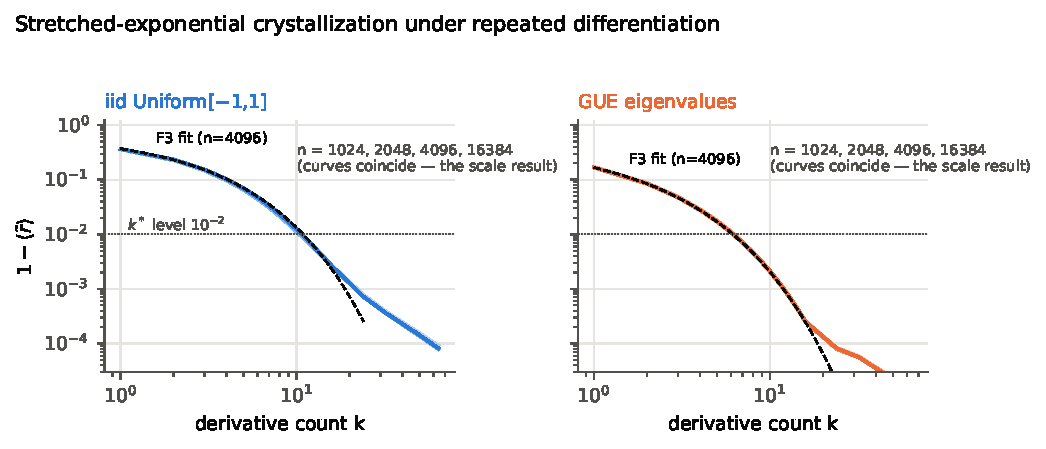
\includegraphics[width=\textwidth]{figs/fig1_relaxation.pdf}
\caption{Relaxation of the gap-ratio distance $\gapdist$ for both seed classes across degrees,
with ensemble $\sigma$ bands and the fitted stretched exponential (F3). The visible departure of
F3 at the largest $n$ is the misfit reported as a finding in \S4: the instrument's precision
improves faster than the three-form family's fidelity.}
\label{fig:relaxation}
\end{figure}

\paragraph{Form.} F3 (stretched exponential, $\gapdist\approx a\exp(-(k/\tau)^{\beta})$) is
selected for both seed classes on all three instrument bands at every $n$ --- decisively by AICc
(margins of $10^2$--$10^3$ against the exponential and power-law alternatives). Stated with its
grade: F3 is AICc-best of the pre-registered ladder, not a demonstrated law. The selected fits
carry residual structure beyond the ensemble $\sigma$ --- $\chi^2/\mathrm{dof}$ rises
$0.76\to2.29\to3.76\to23.4$ along $n=1024\to16384$ on the iid primary arm (raw arms up to
${\sim}98$; the GUE primary is underdispersed at $0.02$--$0.22$, the fingerprint of cross-$k$
correlation from shared replicates). This growth is itself a finding: the instrument's precision
improves faster than the three-form family's fidelity, so at $n=16384$ the measurement resolves
structure beyond F3. That is the quantitative form of ``best-of-three,'' and it is the opening
datum for any richer-form successor.

\paragraph{Rate.} The comparison statistic is $\kstar$, the level crossing at which the fitted
curve reaches $10^{-2}$ --- defined identically for every form in the ladder, and therefore
the one shape quantity that is commensurable across fits that may differ in window or form.
At $n=4096$, $\kstar_{\mathrm{iid}}=10.89$ and $\kstar_{\mathrm{gue}}=6.16$: a Poisson seed
takes roughly eleven derivatives to crystallize and a GUE seed roughly six. The separation
$|\kstar_{\mathrm{iid}}-\kstar_{\mathrm{gue}}|$ is the result of this section, and it is
robust in the sense that matters --- across $15$ defensible choices of fit window (both
edges varied) it moves by $6.1\%$, $7.8\%$ and $6.3\%$ at $n=4096$, $2048$ and $1024$, and
it clears the sealed $5\sigma$ bar under every one of them at every $n$ (bootstrap errors
throughout).\footnote{Reframed 2026-09-15. An earlier draft of this section led with the
shape-parameter significances $z(\tau)$ and $z(\beta)$, which are reported below. They are
correct as computed, but they are window-dependent by one to two orders of magnitude while
the separation is not, and a statistic that moves that much under a nuisance choice is a
diagnostic of the choice rather than a result. The separation is therefore promoted to the
lead and the significances demoted to a sensitivity finding. Nothing about the verdict
changes; what changes is which number a reader is asked to weight.} \textbf{Verdict:}
\verdict{rate-seed-dependent}.

\paragraph{Shape parameters, and their sensitivity.} At $n=4096$ on the primary readout, iid $(\tau=1.734,\ \beta=0.788)$
versus GUE $(0.888,\ 0.703)$: $z(\tau)=20.4$, $z(\beta)=9.3$ against the sealed $5\sigma$
threshold. Under a conservative treatment --- rescaling each covariance by
$\max(1,\chi^2/\mathrm{dof})$ --- $z=12.0$ and $5.84$: the verdict survives, with $z(\beta)$ near
the bar, and both numbers are reported so the reader can weight them.\footnote{A subsequent
error-model study (2026-09-08) recovered the per-replicate curves --- never banked --- and
propagated the replicate-sharing covariance explicitly. $z(\beta)$ clears the sealed $5\sigma$
bar under all seven treatments examined (bootstrap $8.24$; GLS with shrinkage $9.97$--$11.12$;
sealed $9.31$; conservative $5.84$), so the margin is not an artifact of the independent-$\sigma$
assumption. That study's own stability bar was \emph{missed}: the GLS and bootstrap treatments
disagree by up to $35\%$ in $z$-magnitude against a pre-set $25\%$ ceiling, so what it licenses is a
range, not a point value. The direction of the correlation effect is class-dependent and was
predicted before the run: sharing replicates \emph{tightens} $\beta$ for GUE (ratio $0.735$) and
\emph{loosens} it for iid ($1.363$).} The quoted parameter values are
readout-definition- and $n$-dependent (the deliberately biased raw arms give lower
$(\tau,\beta)$; iid $\tau$ scatters ${\sim}0.19$ across $n$); what is robust across every band and
every $n$ is the ordering --- iid $>$ GUE in both $\tau$ and $\beta$ in all 12 band $\times$
degree comparisons, with $\Delta\tau=0.63$--$0.85$ on the primary arm ($0.39$--$0.85$ across all
bands) far exceeding the drift.\footnote{Corrected 2026-08-16, packaging audit: the earlier
``$0.65$--$0.85$'' did not trace --- the $n=2048$ primary cell gives $0.628$. The artifacts are
authoritative; the prose was the defective slot.} 

\paragraph{The significances are a window diagnostic.} The fit window is set by a
threshold, $\text{mean}>10^{-3}$ on the full ensemble, and that threshold lands in a different
place for each class --- iid is fitted on $16$ points, GUE on $11$. Refitting both classes over a
surface of $15$ defensible window rules (lower edge $k_{\mathrm{lo}}\in\{1,\dots,5\}$, upper edge
by the sealed threshold or at a shared $k\le11$ or $k\le16$) separates two quantities that the
paragraph above reports together:

\begin{table}[h]
\centering
\small
\begin{tabular}{lccccc}
\toprule
$n$ & $|\kstar_{\mathrm{iid}}-\kstar_{\mathrm{gue}}|$ & spread & $z(\beta)$ range & swing &
sealed $z(\beta)$ \\
\midrule
1024 & 4.4302--4.7175 & 6.3\% & 0.04--4.58 & $108.9\times$ & 3.80 \\
2048 & 4.0044--4.3311 & 7.8\% & 0.36--5.46 & $15.1\times$ & 3.11 \\
4096 & 4.4443--4.7277 & 6.1\% & 0.12--11.27 & $95.6\times$ & 9.31 \\
\bottomrule
\end{tabular}
\end{table}

\noindent
The \emph{separation} is robust: it moves by $6$--$8\%$ across every window rule at every $n$.
The \emph{significance} is not: $z(\beta)$ moves by one to two orders of magnitude over the same
rules, and the sealed window sits at the $87$th percentile of that range at all three
$n$.\footnote{\emph{Corrected 2026-09-14}: that percentile, and the equality of it across $n$,
are artifacts of the diagonal \texttt{absolute\_sigma} error model these $z$ were computed with.
Recomputed with a replicate bootstrap --- which carries the across-$k$ correlation that error
model omits --- the sealed window sits at $0.93$, $0.47$ and $0.87$ at $n=1024$, $2048$ and
$4096$, i.e.\ at the \emph{median} at $n=2048$. The window sensitivity itself survives the
correction (the swing is $98.3\times$, $11.4\times$ and $42.9\times$ under bootstrap errors), but
it is not true that the threshold rule places the sealed window favourably at every $n$. The
$z$ values quoted in this paragraph are the covariance-model ones throughout; the
bootstrap column is in \texttt{stage3d\_error\_model.json}.} The sealed $z(\beta)$ is also not stable in $n$: $3.80$, $3.11$ and
$9.31$ at $n=1024$, $2048$ and $4096$, so two of the three sizes sit below the $5\sigma$ bar
under the identical rule.\footnote{Measured 2026-09-14. The lower edge is the sensitive one and
is the axis a first attempt failed to declare: the separation is flat in it while $z$ is not,
because dropping iid's $k=1..3$ removes the points that identify $(\tau,\beta)$ --- and those are
exactly the points F3 fits worst (residuals $-1.77,+2.59,+1.90$). Holding F3 fixed is not
question-begging: it is AICc-best on all $24$ (class, window, $n$) cells by margins of $10.3$ to
$5642$.}

This is why the section leads with the separation. The window sensitivity of $z(\beta)$ is
larger than the covariance-treatment sensitivity disclosed above, and it does not touch
\verdict{rate-seed-dependent}: the classes separate under every window rule tested, at every
$n$. A referee who varies the window will reproduce the swing immediately; the point of
reporting it here is that they should also reproduce the $6$--$8\%$ stability of
$|\Delta\kstar|$, which is the claim.

One further caution on the error model, since the $z$ above are quoted from it. The
\texttt{absolute\_sigma} covariance treats the supplied $\sigma$ as exact, so a growing
$\chi^2/\mathrm{dof}$ --- $0.76$, $2.29$, $3.76$ for iid at $n=1024$, $2048$, $4096$ --- does not
widen it. The ratio of covariance-model to bootstrap $z(\beta)$ at the sealed window tracks that
growth: $0.67$, $0.89$, $1.12$. Neither error model is correct at both ends of the window: the
covariance sees the $(\tau,\beta)$ degeneracy on short windows (correlation $0.999$ on seven
points) and is blind to the across-$k$ replicate correlation and to misspecification; the
bootstrap sees the correlation and part of the misspecification, and is blind to the
degeneracy because sixteen near-identical replicates do not explore it. The separation at
$\kstar$ is reported with bootstrap errors because it is not degenerate in the way the shape
parameters are.

\textbf{Verdict:} \verdict{rate-seed-dependent}.

\begin{figure}[t]
\centering
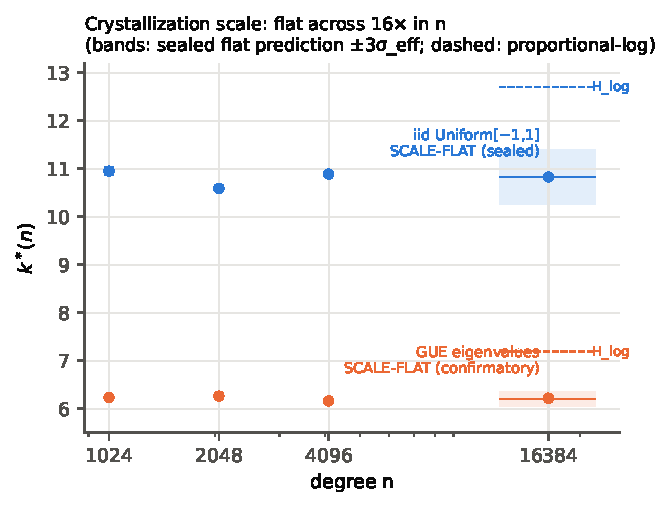
\includegraphics[width=0.85\textwidth]{figs/fig2_kstar.pdf}
\caption{$\kstar(n)$ with the sealed point predictions and their acceptance bands. The
discrimination is between flat-plus-scatter and proportional-log; tuning is impossible by commit
order.}
\label{fig:kstar}
\end{figure}

\paragraph{Scale.} Two point predictions were sealed before the $n=16384$ run from the three
smaller anchors: $H_{\mathrm{flat}}=10.827$ (precision-weighted mean, with $\ssys=0.192$
absorbing the anchors' real scatter --- they are mutually inconsistent as an exact constant,
$\chi^2=27.9/2$ iid and $44.0/2$ GUE, both filed) and $H_{\log}=12.704$ (proportional growth
anchored at $n=4096$; an affine log fit is non-identifiable on near-flat anchors and was rejected
in the seal itself). Measured: $\kstar(\text{iid},16384)=10.828\pm0.011$ --- $0.003\seff$ from
$H_{\mathrm{flat}}$, $9.8\seff$ from $H_{\log}$. \textbf{Verdict:} \verdict{scale-flat}. The GUE
arm, run unsealed-confirmatory, read $6.220\pm0.004$ against its flat prediction $6.202$
($0.34\seff$; log excluded at $18.6\seff$). What these landings certify is the discrimination ---
flat accepted, proportional-log excluded, tuning impossible by commit order. The three-decimal
iid coincidence itself is luck under our own error model ($\seff$ is anchor-scatter-dominated; a
$0.001$ landing has ${\sim}0.4\%$ probability) and is claimed as nothing more; the fit errors
$\sigma_m$ are optimistic (see Form), which is why the sealed adjudication runs on $\seff$
throughout --- the GUE landing sits at $4.2\sigma_m$ and is accepted precisely because the seal's
error model anticipated that $\ssys$ dominates.

\paragraph{Ceiling, floor, and controls.} The Hermite seed's bulk is measured crystalline at
every flow time ($\gapdist$ at $10^{-7}$--$10^{-5}$ --- the finite-$n$ ceiling arm); the picket
fence is ceiling-invariant through the full corrected pipeline at every $k$ and $n$ (the sealed
clause that once fired on the artifact now holds); and the $k=O(1)$ floor --- a Poisson-gapped
seed cannot be crystalline after one Rolle-interlacing step --- is stated as program-derived: the
literature's zero--critical-point pairing theorems require planar densities and exclude real
support by hypothesis.

\section{Discussion}

\paragraph{The two-scale statement.} ANP freeze the macroscopic profile --- asymptotically,
almost surely, for every $k=o(n)$ for real roots, our seed class --- while the local spacing
completes its crystallization by $\kstar\approx6$--$11$, $n$-independent across the measured
range. The mechanistic grounding is the paper's own lemma, offered as interpretation and graded
as such: convex-weight sensitivities decaying quadratically make each root's update a
near-neighbor affair, so relaxation is a local process whose interaction range is measured in
spacings, not fractions of the support --- and a local process has no way to know $n$. Locality
explains why the clock is $O(1)$. It conspicuously fails to explain why the clock is stretched.

\begin{figure}[t]
\centering
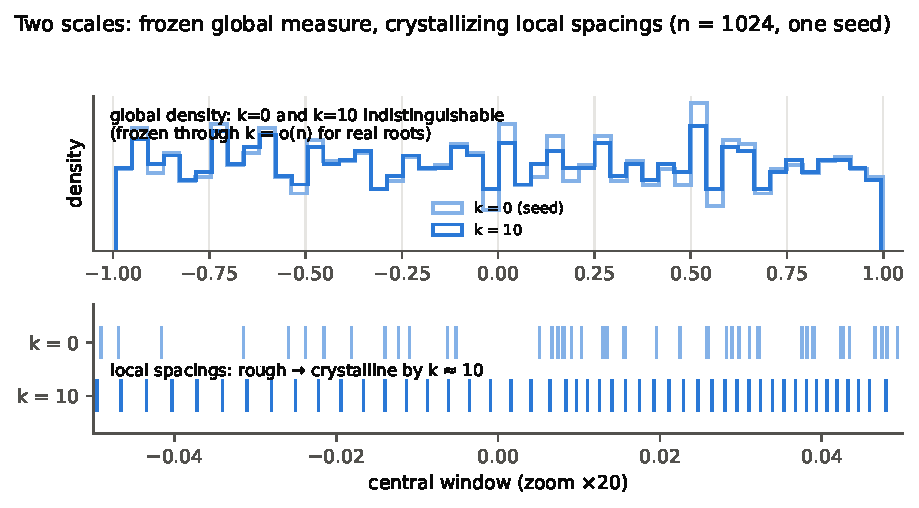
\includegraphics[width=\textwidth]{figs/fig4_twoscale.pdf}
\caption{The two-scale structure: the global measure is asymptotically frozen through every
$k=o(n)$ while local spacing crystallizes by $k\approx10$ beneath it.}
\label{fig:twoscale}
\end{figure}

\paragraph{The stretch.} The selected form, $\exp(-(k/\tau)^{\beta})$ with $\beta<1$, is the
function known as the stretched exponential, or Kohlrausch--Williams--Watts. We use that name
for the function and intend no claim beyond it. This paper does not assert that the derivative
flow is a model of, an analogue of, or evidence about any physical relaxation process, and
nothing below should be read as such a claim; the measurements are of this system only.

What we can state about $\beta<1$ here is a negative, and it is measured rather than argued. The
most immediate account of a stretched relaxation is a mixture: a distribution of local rates
carried by the initial configuration, whose superposition is stretched even though each
component is not. In this system that account fails. Binning roots by their seed gap environment
under rules committed before the data were seen leaves 4 of 5 quintiles stretched; re-binning
mid-flow, on the environment at $k=2$ rather than $k=0$, leaves 3 of 5
($\beta=0.70/0.55/0.49$); and the GUE seed, which is rigid and homogeneous, stretches as much as
the disordered one.\footnote{A later probe (2026-09-08) rebuilt the GUE arm of this experiment,
whose original design left F3 unassessable in most bins (3--4 point windows). Under an adapted
design run identically on both classes, \emph{both} read \verdict{not\_supported} at 5 of 5
bins: what is seed-dependent is the parameters, not the mechanism.} Neither the initial nor the
instantaneous local gap environment carries the rate distribution. The design is of a familiar
shape --- condition on configuration, then ensemble over realization --- though with a
difference worth stating: the flow is deterministic and has no momentum-like variable, so the
ensemble resamples seed-adjacent perturbation at fixed conditioning rather than velocities.

\begin{figure}[t]
\centering
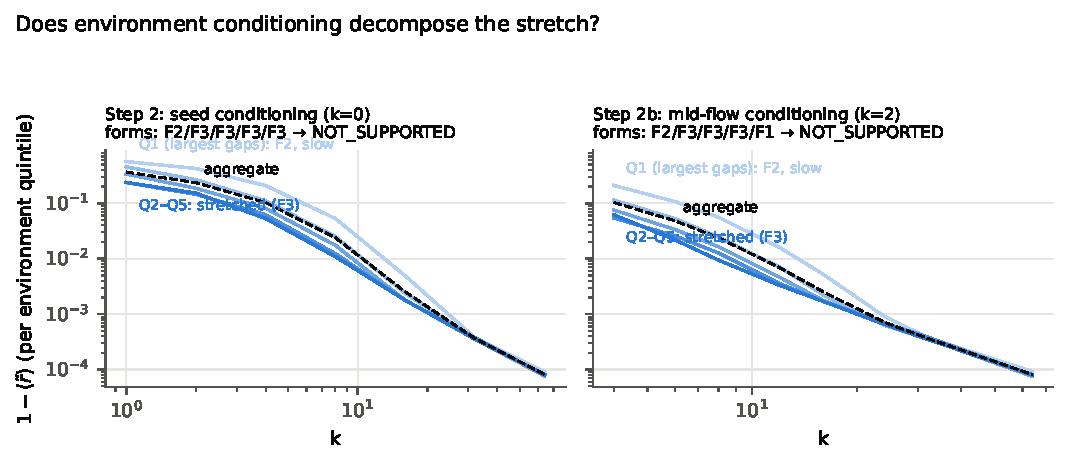
\includegraphics[width=\textwidth]{figs/fig3_bins.pdf}
\caption{Per-bin decomposition by gap environment. Conditioning does not decompose the stretch:
the residual structure lives in the mixture, not the components.}
\label{fig:bins}
\end{figure}

Three textures constrain any candidate mechanism, and we report them without proposing one. A
stable slow subpopulation: the largest-gap quintile selects a pure exponential at both
conditioning times with nearly unchanged rate ($\tau=3.07$ at $k=0$, $3.18$ at $k=2$). An
emergent fast power-law component: the smallest-gap quintile at $k=2$ selects F1,
$\chi^2/\mathrm{dof}=1.2$. And a mixture effect: the per-bin fits at $k=2$ conditioning are
mostly good ($\chi^2/\mathrm{dof}=0.5$--$1.2$ for the middle quintiles) while the aggregate
misfits, so the residual structure lives in the mixture rather than in the components. Rates do
order monotonically by environment ($\kstar=13.63\to8.02$ across quintiles, strictly monotone;
$\tau=3.18\to0.30$ is the same ordering read off a shape parameter, and is quoted only for
continuity with the banked per-bin fits --- see \S\ref{sec:ordering}); what environment fails to
account for is the stretch \emph{within} each bin.

We have no mechanism for $\beta<1$ in this system. That is the paper's open question, and we
state it as open rather than assigning it to any existing account.

\subsection*{Adjacent tracks}

Two global treatments cover the regimes surrounding ours and are recorded here with the searches
that place them. The Hopf-equation approach of Mart\'inez-Finkelshtein--Rakhmanov
(arXiv:2408.13851) is the most general treatment of the global zero flow for $k/n\to t$: it
establishes convergence of the Cauchy transform of the normalized zero-counting measure, with
connections to the inviscid Burgers equation, fractional free convolution, and a nonlocal
diffusion equation for the density. An exhaustive search of its extracted full text returns
\textbf{zero} occurrences of \emph{spacing}, \emph{gap}, \emph{microscopic}, \emph{consecutive
roots}, \emph{fluctuation}, \emph{rigidity}, \emph{point process}, \emph{pair correlation},
\emph{universality}, \emph{nearest neighbour} or \emph{crystalliz}-; all twelve occurrences of
\emph{local} are either the PDE's name (\emph{nonlocal} transport/diffusion, a statement about
the macroscopic density) or \emph{locally uniformly}, a convergence topology.
Arizmendi--Fujie--Perales--Ueda (arXiv:2408.09337) connect repeated differentiation to the
$S$-transform and the finite free cumulants in the proportional and $o(n)$ regimes; the same
search of its full text returns zero for the same terms, with all four occurrences of
\emph{local} being \emph{locally uniform convergence}. Both are global empirical-measure results,
and neither contains a local-spacing statement to compare our curves against --- which is what
makes the gap above a scoped claim rather than an absence of citation.

The endpoint papers are outside our regime by their own statements: Campbell
(\texttt{doi:10.4171/dm/1071}) identifies the limits of repeated differentiation as the real
rooted Appell sequences precisely when \emph{the remaining degree is fixed}, and
Arizmendi--Campbell--Fujie (arXiv:2506.08910) give CLTs in the same endpoint regime; both are
read at abstract-and-structure depth, which is sufficient to place a regime and is stated as the
depth reached. The complex/rotationally-invariant flow (Galligo--Najnudel--Vu; Najnudel--Vu) and
the heat flow (Hall--Ho--Jalowy--Kabluchko, \emph{Indiana Univ.\ Math.\ J.}\ \textbf{74} (2025);
\emph{EJP} \textbf{30} (2025); Hall--Ho, \emph{Lett.\ Math.\ Phys.}\ \textbf{115} (2025)) are
both active; neither touches real-rooted fixed-$k$ local statistics.

Two further rate-shaped results sit adjacent and neither reaches this regime. Kiselev--Tan
(arXiv:2012.09080) rigorously connect root evolution to Steinerberger's PDE for a class of
\emph{trigonometric} polynomials in the periodic setting and obtain \textbf{exponential}
convergence to uniform density --- but in $t=k/n$, the proportional regime, and for the
\emph{density}, a global object; the contrast with a stretched exponential in fixed $k$ for a
\emph{local} statistic is the whole distance between their setting and ours. And the announced
Part~III of the Jalowy--Kabluchko--Marynych program is \textbf{still unposted} as of the
submission-day re-sweep (Part~I, arXiv:2504.11593, April 2025; Part~II, arXiv:2509.11248,
September 2025). Part~I describes Part~III as establishing functional limit theorems for the
random \emph{profiles} of random polynomials, relating profile fluctuations to \textbf{the rate
of convergence of the empirical zero distribution} --- so when it lands it will sharpen a global
object, not a local one.\footnote{An earlier draft of this paragraph called it ``the nearest
theorem-shaped object to our $\sigma$-resolved curves''; on the series' own description that
overstates it, and the sentence is corrected rather than left standing.} Part~II's catalog of
exactly-characterized seed families was the natural extension of the seed roster for mapping the
$(\tau,\beta)$ dependence beyond two classes.

\subsection*{The seed roster, run}

That extension has since been run, on a different roster and with a sharper design (2026-09-09,
exploratory and unsealed; it does not touch the sealed verdict). The JKM families are catalogued
by their \emph{global} shape, and varying global shape would confound the two scales this paper
separates --- so the roster used instead is the $\beta$-Hermite ensembles, for which every member
shares the \textbf{same semicircle global law} while $\beta$ is precisely the repulsion exponent.
The design is therefore matched by construction: local statistics vary, the global measure does
not (verified --- max pairwise seed-law KS $0.0012$). Since the GUE seed used throughout this
paper is already the Dumitriu--Edelman $\beta=2$ tridiagonal, the family generalises by one
parameter and $\beta=2$ reproduces the banked GUE arm to all 40 numbers, making the existing
science run the extension's premise rather than a neighbouring result. The outcome is that
\textbf{the $(\tau,\beta)$ seed-dependence is a surface, and local repulsion is its coordinate}:

\begin{table}[h]
\centering
\begin{tabular}{cccc}
\toprule
$\beta$ (repulsion) & $\kstar$ & $\tau$ & stretch exponent \\
\midrule
1 & 6.9223 & 0.9732 & 0.7172 \\
2 & 6.1628 & 0.8884 & 0.7030 \\
4 & 5.4664 & 0.8031 & 0.6837 \\
\bottomrule
\end{tabular}
\caption{The matched $\beta$-Hermite roster: identical semicircle global law, varying local
repulsion.}
\end{table}

$\kstar$ decreases strictly with repulsion (ends separated by $122.9$ combined $\sigma$), and
$\tau$ and the stretch exponent order with it. The iid seed continues the trend in every
coordinate ($\kstar=10.889$, $\tau=1.734$, stretch $=0.788$) but carries a \emph{different}
global law, so it is an unmatched reference rather than a fourth point on the surface. Two
consequences for this paper's claims: the stretched form is not a property of the GUE seed ---
every member of the roster selects F3 --- and the seed-dependence reported above is not a
two-point accident but a monotone function of a named physical parameter. What the roster does
not supply is a mechanism for the \emph{stretch itself}, which remains what nothing on offer
predicts.

\subsection*{A note on which quantity carries the ordering}
\label{sec:ordering}

The per-bin fits select their functional form independently by AICc, so a $\tau$ compared across
bins is generally compared across \emph{forms} --- and $\tau$ in a stretched exponential is
degenerate with its stretch exponent besides. Re-reading all five per-bin conditionings at
$\kstar$, the level crossing that is defined identically for every form in the ladder, the
environmental ordering is \textbf{strictly monotone in four of the five}, while the $\tau$
readings report it in only one. $\tau$ misses it for two non-physical reasons: an F1 bin yields
no $\tau$ at all, so the ordering is scored on a missing value; and within a uniformly-F3 cell
the $\tau/\beta$ degeneracy alone can shuffle a real ordering. The ordering claim in this paper
is therefore \emph{stronger} than its $\tau$-based statement suggested, and is quoted at $\kstar$
above. No verdict moves: the per-bin ladder's supported branch requires four of five bins to
select the exponential \emph{and} monotone $\tau$, and it never fired in any cell. The one
genuine non-monotonicity is seed-conditioning ($k=0$) in its last quintile only
($\kstar=9.280\to9.337$), which the $\tau$ reading could not have shown.

\appendix

\section{The measurement chain}
\label{app:chain}

The verdict history, with commit hashes, is the paper's honesty appendix. A hostile referee
looking for the weakness should find we published it first.

\begin{table}[h]
\centering
\small
\begin{tabular}{lll}
\toprule
Stage & Commit & Outcome \\
\midrule
v1 verdict, form clause & \texttt{4f29d70} & \verdict{rate-seed-dependent} (v1 instrument) \\
Instrument artifact found & \texttt{c235861} & by the roadmap's own regression step \\
Contamination measured & \texttt{be7f2b9} & fit-window anchors at $24$--$38\smean$ \\
Corrected reference pinned & \texttt{78ce01a} & sight-unseen; failed its own lattice gate \\
Gate-forced amendment & \texttt{c7275d3} & Richardson pair-extrapolation (v1.5.1) \\
Gates re-certified & \texttt{d6a7cff} & downgraded to \verdict{inconclusive-on-instrument-grounds} \\
Dense-grid amendment & \texttt{c986573} & second disclosure ledger and grade label \\
Re-adjudication & \texttt{6cc2562} & \verdict{rate-seed-dependent} via the $z$-clause \\
Scale law sealed & \texttt{d629f6f} & \verdict{scale-flat} (seal \texttt{889f472}) \\
Post-review disclosure & \texttt{505931c} & \\
\bottomrule
\end{tabular}
\end{table}

The downgrade at \texttt{d6a7cff} was earned rather than technical: the original powers-of-two
$k$-grid gave the GUE arm too few points inside its fit window to adjudicate a form, and the
small-sample guard correctly refused. The grid-density amendment changed the grid and nothing
else.

\section{Literature verification protocol}
\label{app:lit}

Two adversarial audits (2026-08-11, four targets, ${\sim}30$ sources; 2026-08-13, ${\sim}55$
sources, including full-text silence checks on ANP and citation-graph sweeps of both rail
papers), and a submission-day re-sweep, dated at execution, so that the paper's open-regime
claims carry their verification date.

A process fact is filed openly: the 08-13 audit found a paper our earlier sweeps had missed for
eleven months (JKM Part~II, posted 2025-09) --- global-only, gap intact --- which is why the
re-sweep re-runs the searches rather than citing prior audits. The open-regime claim is therefore
always ``as of [date], verified by [protocol],'' never a standing fact. The submission-day
re-sweep confirmed: Part~III still unposted; Kiselev--Tan added as an adjacent rate result; no
new work reaching local spacing statistics in this regime.

\section{Reproducibility and cost}
\label{app:repro}

Wall-clock economics for replicators: the $n=16384$ arm ran 16 replicates on a Ryzen 5900X under
5-way replicate-level multiprocessing and netted ${\sim}1.5$--$2\times$ over serial --- these
kernels are streaming-dominated (${\sim}3$ flops/byte), so the memory-bandwidth wall binds well
below the core count; budget accordingly. Solver temporaries are candidate-axis-chunked
(bitwise-identical; known-answer gates re-certified after the change, per the seal's post-change
protocol). All RNG derives from a single committed \texttt{SeedSequence} master; every replicate
is enumerable in advance and every run is exactly reproducible, including across the two OS
reboots this campaign absorbed mid-flight.

Two disclosed limitations. The dense-grid and $16384$ artifacts bank per-$k$ ensemble statistics
but not per-replicate readouts (an internal-rule violation caught in review; per-replicate
$\kstar$ error estimation would need a re-run).\footnote{Those per-replicate curves were
subsequently recovered by re-running the sealed flows, which reproduced the banked artifact
exactly (0 of 80 numbers mismatched); see the error-model footnote in \S4.} And $\ssys$ --- a
3-point anchor standard deviation, itself uncertain by ${\sim}\pm50\%$ --- enters the scale
adjudication as a Gaussian in quadrature, a disclosed modeling choice. The anchors are mutually
inconsistent as an \emph{exact} constant ($\chi^2=27.9/2$ iid, $44.0/2$ GUE, both filed):
\verdict{scale-flat} is a two-hypothesis discrimination between flat-plus-scatter and
proportional-log, never a claim that $\kstar$ is constant.

\end{document}
